\section{Korrektur zur Auswertung des 1-dimensionaler Festkörpers}
\subsection{Unterschiedliche Blenden}
Die Auswertung des 1-dimensionaler Festkörpers hat mit unseren Daten in Kapitel
\ref{sec:1dimFK} nicht geklappt.
An dieser Stelle werden die Ergebnisse des Protokolls von Lothar Brosda und
Eiko Evers vom 06. Juli 2014 verwendet.

Die Abbildung \ref{fig:1dkorrektur} zeigt deutlich,
dass bei einer höheren Anzahl an Zylindern die Kurve mehr Maxima und Minima aufweist.
Die Blendengröße hat einen Einfluss auf die Position der Maxima und auf die Amplitude.
\begin{figure}
  \centering
  \caption{Plots für verschiedene Anzahlen an Zylindern der Länge $L=\SI{50}{\milli\meter}$ und Blendengrößen.}
  \label{fig:1dkorrektur}
  % 10mm Blende
  \begin{subfigure}{0.3\textwidth}
    \centering
    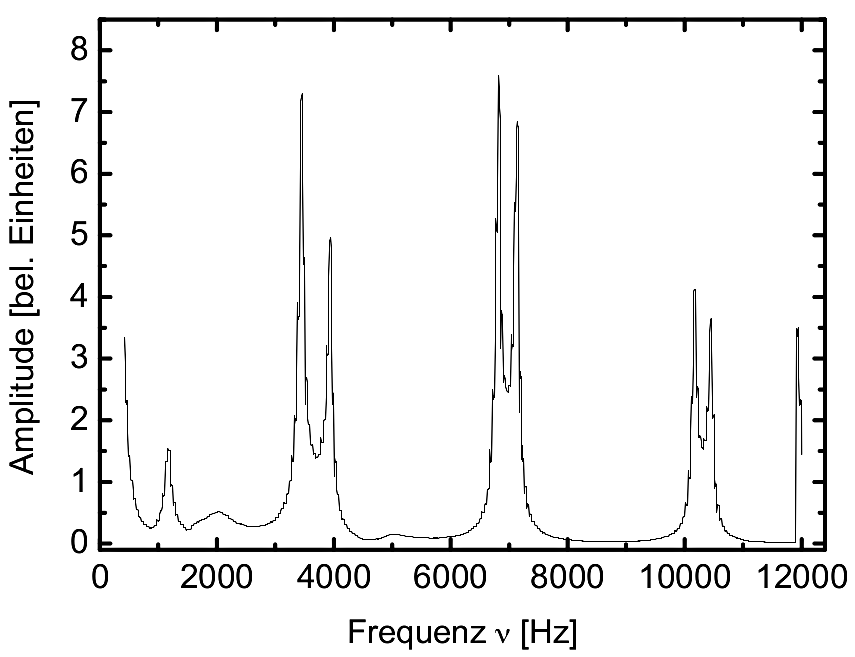
\includegraphics[width=\textwidth]{korrektur/2_50mm_10.png}
    \caption{Zwei Zylinder,\\$\SI{10}{\milli\meter}$-Blende.}
  \end{subfigure}
  \begin{subfigure}{0.3\textwidth}
    \centering
    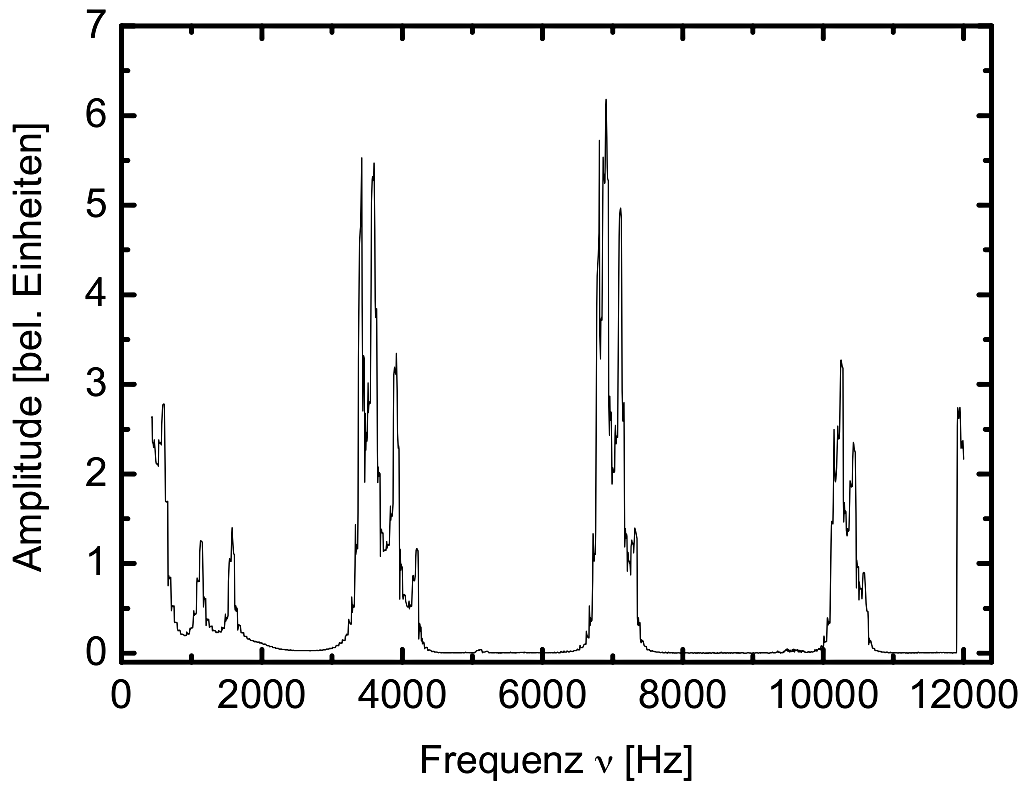
\includegraphics[width=\textwidth]{korrektur/4_50mm_10.png}
    \caption{Vier Zylinder,\\$\SI{10}{\milli\meter}$-Blende.}
  \end{subfigure}
  \begin{subfigure}{0.3\textwidth}
    \centering
    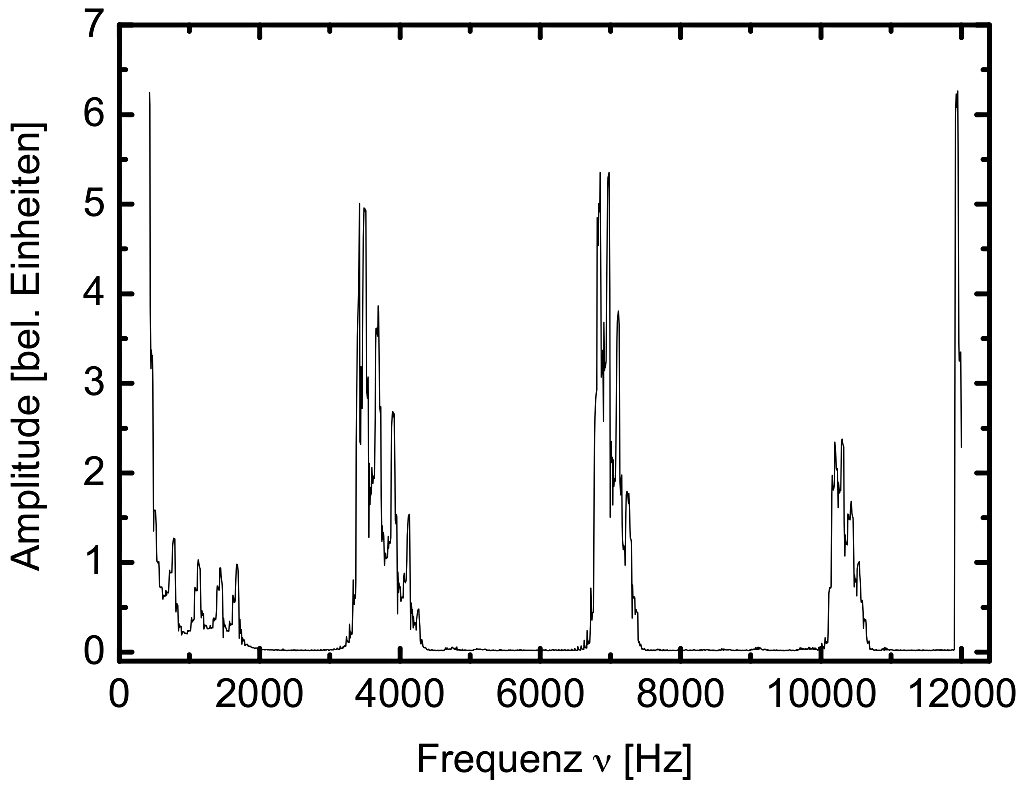
\includegraphics[width=\textwidth]{korrektur/6_50mm_10.png}
    \caption{Sechs Zylinder,\\$\SI{10}{\milli\meter}$-Blende.}
  \end{subfigure}
  % 13mm Blende
  \begin{subfigure}{0.3\textwidth}
    \centering
    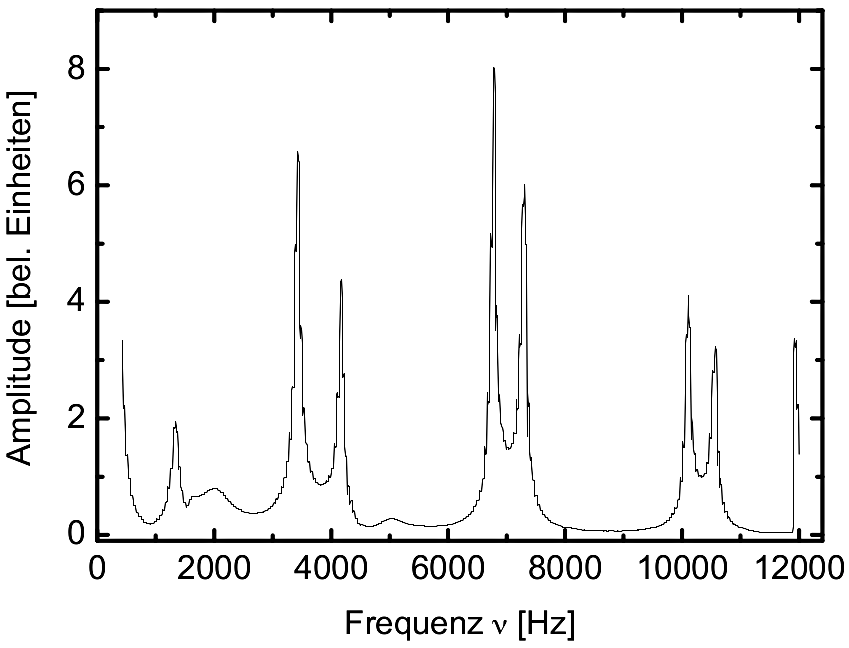
\includegraphics[width=\textwidth]{korrektur/2_50mm_13.png}
    \caption{Zwei Zylinder,\\$\SI{13}{\milli\meter}$-Blende.}
  \end{subfigure}
  \begin{subfigure}{0.3\textwidth}
    \centering
    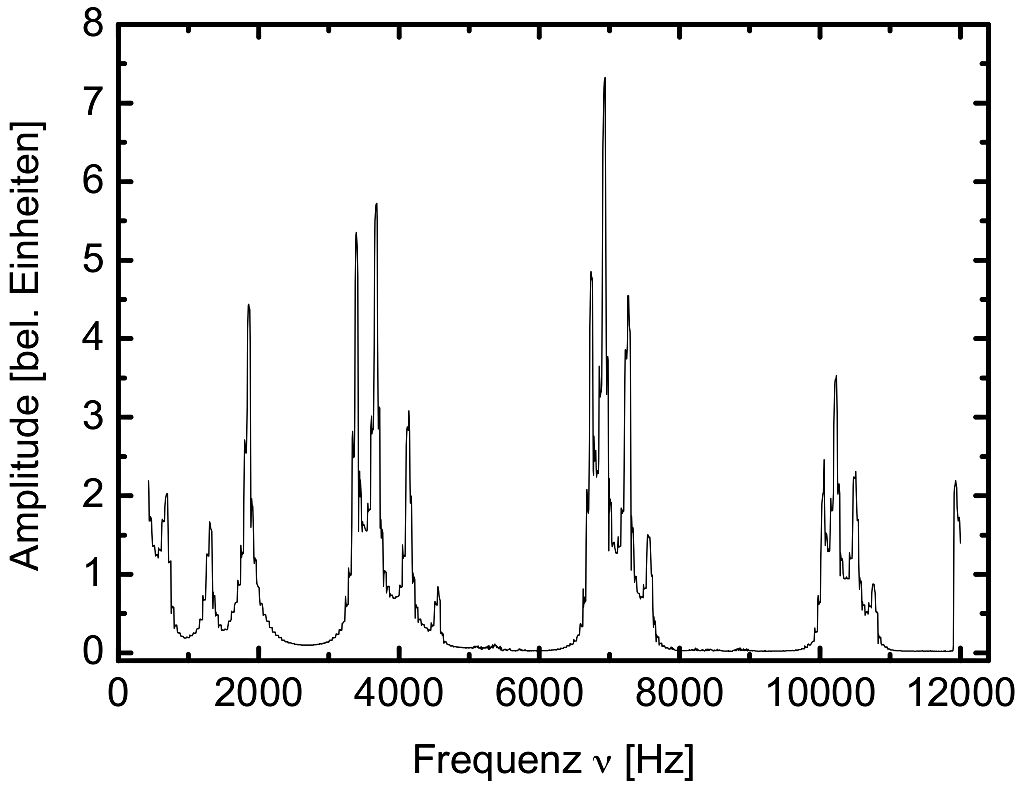
\includegraphics[width=\textwidth]{korrektur/4_50mm_13.png}
    \caption{Vier Zylinder,\\$\SI{13}{\milli\meter}$-Blende.}
  \end{subfigure}
  \begin{subfigure}{0.3\textwidth}
    \centering
    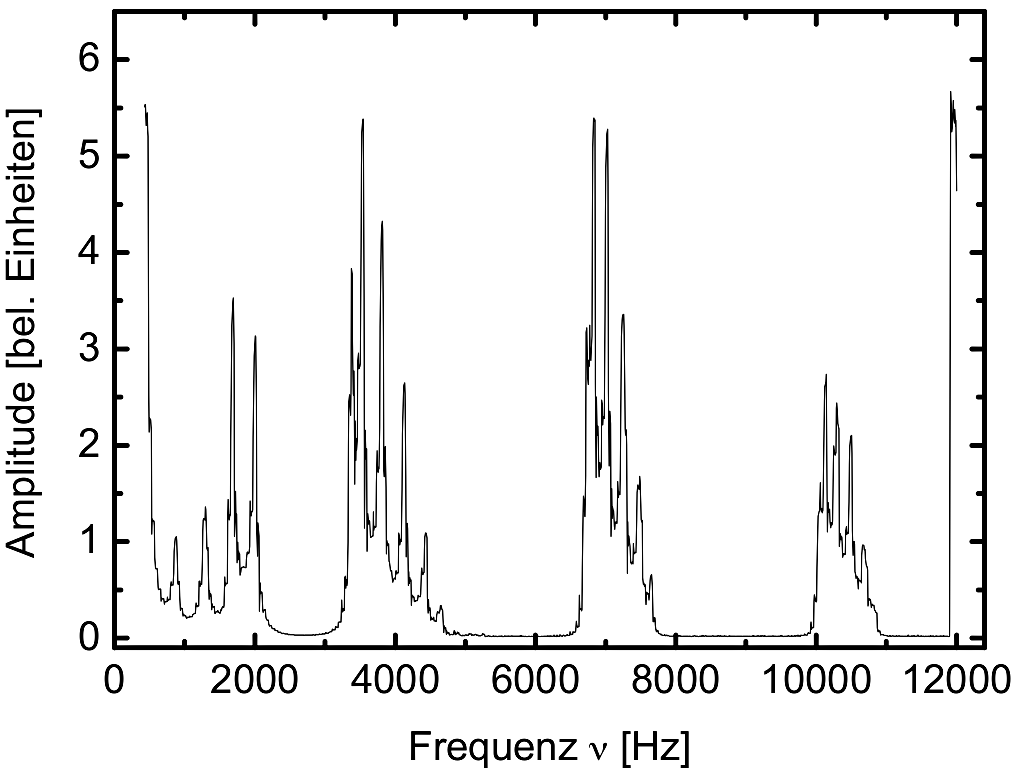
\includegraphics[width=\textwidth]{korrektur/6_50mm_13.png}
    \caption{Sechs Zylinder,\\$\SI{13}{\milli\meter}$-Blende.}
  \end{subfigure}
  % 16mm Blende
  \begin{subfigure}{0.3\textwidth}
    \centering
    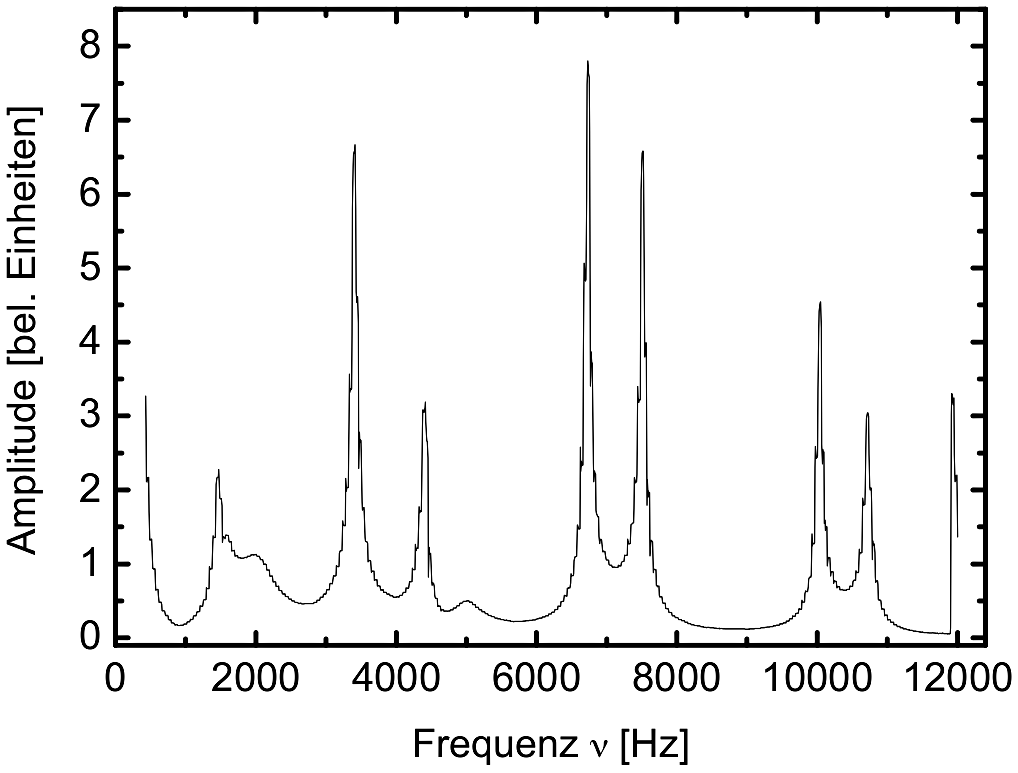
\includegraphics[width=\textwidth]{korrektur/2_50mm_16.png}
    \caption{Zwei Zylinder,\\$\SI{16}{\milli\meter}$-Blende.}
  \end{subfigure}
  \begin{subfigure}{0.3\textwidth}
    \centering
    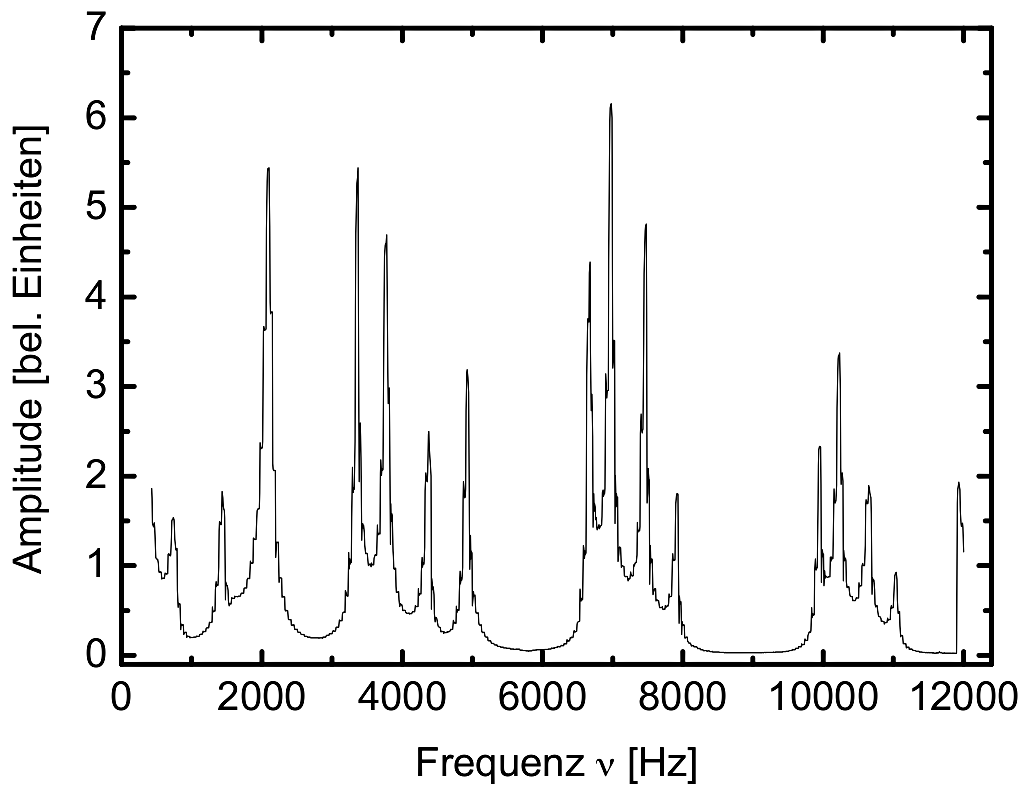
\includegraphics[width=\textwidth]{korrektur/4_50mm_16.png}
    \caption{Vier Zylinder,\\$\SI{16}{\milli\meter}$-Blende.}
  \end{subfigure}
  \begin{subfigure}{0.3\textwidth}
    \centering
    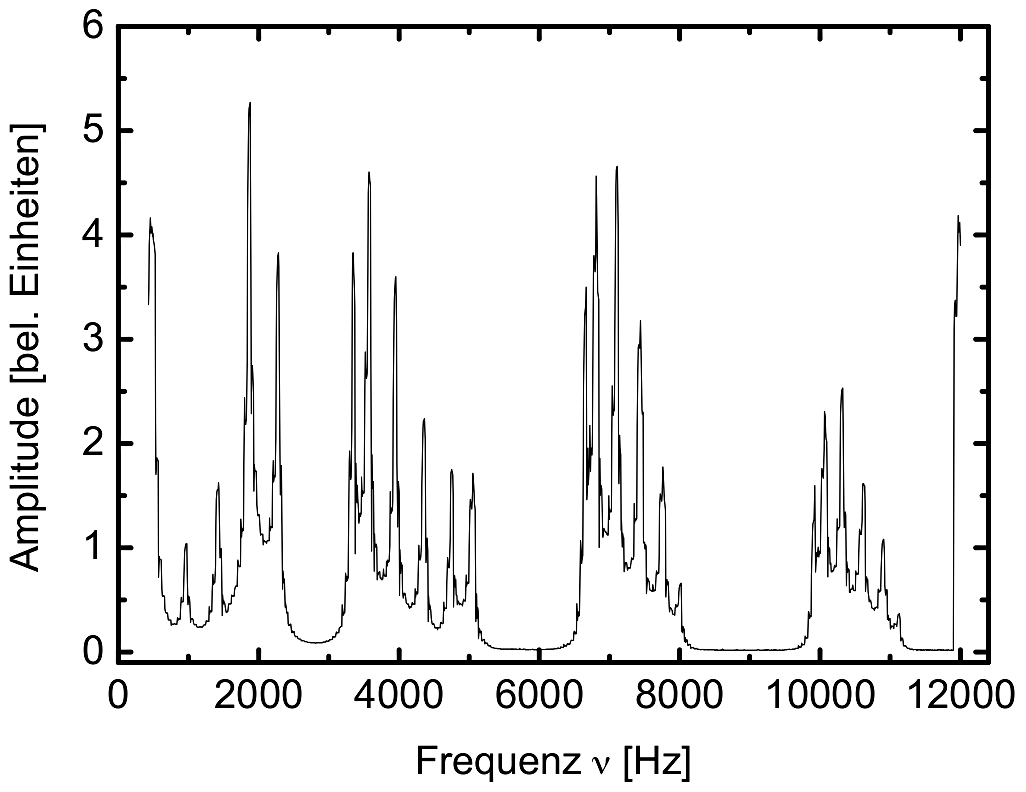
\includegraphics[width=\textwidth]{korrektur/6_50mm_16.png}
    \caption{Sechs Zylinder,\\$\SI{16}{\milli\meter}$-Blende.}
  \end{subfigure}
\end{figure}

\FloatBarrier
\subsection{Zylinderaustausch}
Abbildung \ref{fig:korrekturtausch} zeigt die Frequenzspektren die gemessen werden sollten,
wenn in der Kette aus zwölf $\SI{50}{\milli\meter}$-Zylindern einer gegen einen
$\SI{75}{\milli\meter}$ langen oder einen $\SI{25}{\milli\meter}$ langen Zylinder ausgetauscht wird.

\begin{figure}
  \centering
  \caption{Plots der Frequenzspektren bei Vertauschung der Zylinder.}
  \label{fig:korrekturtausch}
  \begin{subfigure}{0.49\textwidth}
    \centering
    \includegraphics[width=\textwidth]{daten_von_eiko/Defekt/4_12_seg3_25mm.eps}
    \caption{$\SI{25}{\milli\meter}$-Zylinder an Position 3.}
  \end{subfigure}
  \begin{subfigure}{0.49\textwidth}
    \centering
    \includegraphics[width=\textwidth]{daten_von_eiko/Defekt/4_12_seg3_75mm.eps}
    \caption{$\SI{75}{\milli\meter}$-Zylinder an Position 3.}
  \end{subfigure}
  \begin{subfigure}{0.49\textwidth}
    \centering
    \includegraphics[width=\textwidth]{daten_von_eiko/Defekt/4_12_seg6_25mm.eps}
    \caption{$\SI{25}{\milli\meter}$-Zylinder an Position 6.}
  \end{subfigure}
  \begin{subfigure}{0.49\textwidth}
    \centering
    \includegraphics[width=\textwidth]{daten_von_eiko/Defekt/4_12_seg6_75mm.eps}
    \caption{$\SI{75}{\milli\meter}$-Zylinder an Position 6.}
  \end{subfigure}
  \begin{subfigure}{0.49\textwidth}
    \centering
    \includegraphics[width=\textwidth]{daten_von_eiko/Defekt/4_12_seg9_25mm.eps}
    \caption{$\SI{25}{\milli\meter}$-Zylinder an Position 9.}
  \end{subfigure}
  \begin{subfigure}{0.49\textwidth}
    \centering
    \includegraphics[width=\textwidth]{daten_von_eiko/Defekt/4_12_seg9_75mm.eps}
    \caption{$\SI{75}{\milli\meter}$-Zylinder an Position 9.}
  \end{subfigure}
\end{figure}
